\documentclass[11pt]{article}

\usepackage[a4paper,margin=1in]{geometry}
\usepackage{titlesec}
\usepackage{enumitem}
\usepackage{array}
\usepackage{booktabs}
\usepackage{longtable}
\usepackage{tikz}
\usetikzlibrary{arrows.meta, positioning, fit, backgrounds}
\usepackage{xcolor}
\usepackage{parskip}
\usepackage{fancyhdr}
\usepackage[colorlinks=true, linkcolor=blue, urlcolor=blue, citecolor=blue]{hyperref}

\definecolor{srsgray}{RGB}{90,90,90}

\hypersetup{
  pdftitle={AutoQP -- Software Requirements Specification},
  pdfauthor={Development Team},
  pdfsubject={Software Requirements Specification, IEEE Std 830-1998}
}

\newcommand{\priority}[1]{\textbf{Priority:} #1}
\newcommand{\reqid}[1]{\textbf{#1}}

\titleformat{\section}{\Large\bfseries}{\thesection}{0.6em}{}
\titleformat{\subsection}{\large\bfseries}{\thesubsection}{0.6em}{}
\titleformat{\subsubsection}{\bfseries}{\thesubsubsection}{0.6em}{}

\pagestyle{fancy}
\fancyhf{}
\fancyhead[L]{\small\color{srsgray} AutoQP --- Software Requirements Specification}
\fancyhead[R]{\small\color{srsgray} \thepage}
\renewcommand{\headrulewidth}{0.4pt}
\renewcommand{\headrule}{\hbox to\headwidth{\color{srsgray}\leaders\hrule height \headrulewidth\hfill}}

\begin{document}

% =====================================================================
% TITLE PAGE
% =====================================================================
\begin{titlepage}
\thispagestyle{empty}
\begin{center}
\vspace*{2.2cm}

{\small\color{srsgray}\MakeUppercase{Software Requirements Specification}}\\[0.35cm]
{\color{srsgray}\rule{0.42\linewidth}{0.4pt}}\\[1.4cm]

{\Huge\bfseries AutoQP}\\[0.5cm]
{\Large Centralized AI-Assisted Exam Question Bank\\ \& Compilation Platform}\\[1.8cm]

{\color{srsgray}\rule{0.6\linewidth}{0.4pt}}\\[1cm]

{\normalsize Prepared in accordance with IEEE Std 830-1998}\\[0.15cm]
{\normalsize\emph{IEEE Recommended Practice for Software Requirements Specifications}}

\vfill

{\normalsize Document Version 1.1}\\[0.15cm]
{\normalsize September 11, 2026}\\[0.5cm]
{\normalsize Development Team}

\vspace*{1.8cm}
\end{center}
\end{titlepage}

% =====================================================================
% REVISION HISTORY
% =====================================================================
\thispagestyle{empty}
\section*{Revision History}
\addcontentsline{toc}{section}{Revision History}

\begin{longtable}{@{}p{1.6cm}p{2.6cm}p{7.6cm}p{2.6cm}@{}}
\toprule
\textbf{Version} & \textbf{Date} & \textbf{Description} & \textbf{Author} \\
\midrule
\endhead
1.0 & Aug 31, 2026 & Initial baseline release. & Development Team \\[4pt]
1.1 & Sep 11, 2026 & Reclassified Question Forking / Duplication from Low
  to Medium priority, now REQ-11.1 (rationale: it mitigates the same
  shared-bank integrity risk as Concurrency Auditing, and its marginal
  implementation cost is low). Removed references to implementation-level
  project artifacts to keep this specification self-contained. Title page
  redesigned. & Development Team \\
\bottomrule
\end{longtable}

\newpage
\pagestyle{fancy}
\tableofcontents
\newpage

% =====================================================================
\section{Introduction}
% =====================================================================

\subsection{Purpose}
This Software Requirements Specification (SRS) describes the functional and
non-functional requirements of AutoQP, a centralized web platform that
allows instructors to generate, extract, review, store, and assemble exam
questions, and compile them into publication-quality PDF question papers via
an automated LaTeX-based document engine. This document is intended to serve
as the authoritative reference for what the system must do, for use by the
development team, the course instructor acting as project sponsor, and any
future maintainer of the codebase. It specifies required behavior, not
implementation: database schema design, API contracts, and coding
conventions are addressed by separate project artifacts and are outside the
scope of this document, except where a specific technology choice is itself
a binding constraint on requirements (see Section~2.5).

\subsection{Document Conventions}
Requirements are numbered \texttt{REQ-\textless feature\textgreater.\textless
index\textgreater} (e.g. \texttt{REQ-1.2}) and grouped by system feature in
Section~4. Each feature is assigned one of three priority levels, mapped from
the project's MoSCoW prioritization:

\begin{center}
\begin{tabular}{@{}ll@{}}
\toprule
\textbf{Priority in this SRS} & \textbf{MoSCoW equivalent} \\
\midrule
High & Must-Have \\
Medium & Should-Have \\
Low & Could-Have \\
\bottomrule
\end{tabular}
\end{center}

Features marked \emph{Wish List} in the originating project outline are
explicitly excluded from this SRS (see Section~1.4) and are not assigned
requirement IDs. The keywords \textbf{shall} (mandatory), \textbf{should}
(recommended but not mandatory), and \textbf{may} (optional) are used per
IEEE 830 convention to indicate the binding strength of each requirement.

\subsection{Intended Audience and Reading Suggestions}
\begin{itemize}[nosep]
  \item \textbf{Development team members} should read Sections~2--4 in full
    before implementing any feature, and treat Section~4's priority tags as
    the binding delivery order (High before Medium before Low).
  \item \textbf{The course instructor / project sponsor}, evaluating this as
    a course deliverable, may read Sections~1--2 for scope and Section~4's
    feature descriptions without needing the full functional requirement
    lists.
  \item \textbf{Future maintainers} should treat Section~5 (non-functional
    requirements) and Appendix~A (data model) as load-bearing constraints,
    not suggestions.
\end{itemize}

\subsection{Product Scope}
AutoQP replaces manual, word-processor-based exam typesetting with a
centralized, subject-partitioned question bank and an automated document
compilation pipeline. In scope: AI-assisted question generation, extraction
of questions from pasted text and screenshots, a human-review staging area,
a searchable shared repository, automated exam blueprint assembly, and
LaTeX-based PDF compilation with a raw markup source. Out of scope for this
version: any student-facing functionality (submission, auto-grading, a
student portal), multi-institution moderation/approval chains, full-page
computer-vision ingestion of scanned multi-column exams, and semantic
duplicate detection via embeddings. These exclusions correspond to the
``Wish List'' tier of the originating project outline and were confirmed
out of scope by the project's feasibility review (see Section~1.5).

\subsection{References}
\begin{itemize}[nosep]
  \item IEEE Std 830-1998, \emph{IEEE Recommended Practice for Software
    Requirements Specifications}.
  \item Project Outline and MoSCoW Feature Breakdown (originating
    requirements brief supplied by the project sponsor).
  \item Project Feasibility Report (Technical, Operational, Economic, Time,
    Social, Legal, Market, and Resource feasibility findings).
\end{itemize}

% =====================================================================
\section{Overall Description}
% =====================================================================

\subsection{Product Perspective}
AutoQP is a new, standalone product; it is not a modification of an
existing system. It is intended to replace an informal, ad hoc workflow
(instructors typesetting exams individually in Microsoft Word or similar
word processors) with a shared, centrally managed platform. Figure~1 shows
the system's high-level architecture: a browser-based client communicates
exclusively with an application server, which is the sole component
authorized to communicate with the database, the AI provider, and the
document compilation service.

\begin{figure}[h]
\centering
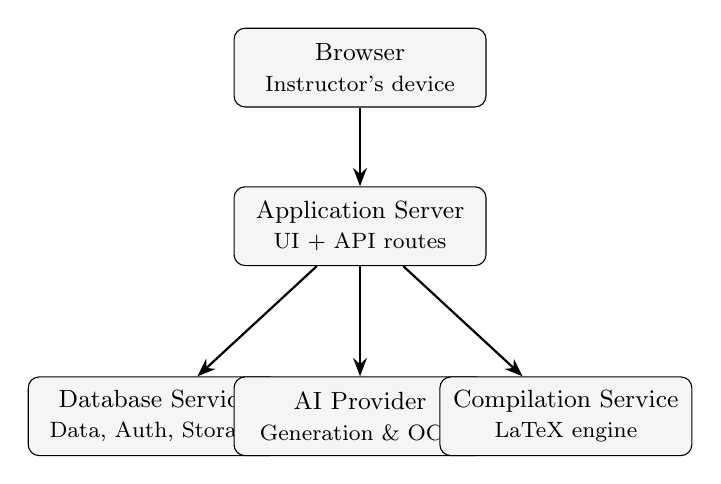
\begin{tikzpicture}[
  node distance=10mm and 12mm,
  box/.style={draw, rounded corners, minimum width=32mm, minimum height=10mm,
    align=center, font=\small, fill=gray!8},
  arr/.style={-Stealth, thick}
]
\node[box] (browser) {Browser\\\footnotesize Instructor's device};
\node[box, below=of browser] (server) {Application Server\\\footnotesize UI + API routes};
\node[box, below left=14mm and -6mm of server] (db) {Database Service\\\footnotesize Data, Auth, Storage};
\node[box, below=14mm of server] (ai) {AI Provider\\\footnotesize Generation \& OCR};
\node[box, below right=14mm and -6mm of server] (compile) {Compilation Service\\\footnotesize LaTeX engine};

\draw[arr] (browser) -- (server);
\draw[arr] (server) -- (db);
\draw[arr] (server) -- (ai);
\draw[arr] (server) -- (compile);
\end{tikzpicture}
\caption{High-level system architecture.}
\end{figure}

\subsection{Product Functions}
At a high level, the system shall allow an authenticated instructor to:
generate or extract candidate questions; review and edit those candidates
before they enter a shared bank; search and filter the bank by subject,
topic, difficulty, and marks; assemble a paper automatically from a mark
pattern; and compile the assembled paper into a downloadable PDF and its
raw LaTeX source. A full breakdown appears in Section~4.

\subsection{User Classes and Characteristics}
\begin{description}[leftmargin=!,labelwidth=3.2cm]
  \item[Instructor] The primary user class. Assumed to be subject-matter
    experts with no assumed programming or LaTeX background. Interacts with
    the system to generate, review, bank, and assemble questions into
    papers scoped to the subjects they are assigned to.
  \item[Administrator] A secondary user class responsible for creating
    subjects and assigning instructors to them. Assumed to have the same
    technical background as an Instructor; distinguished only by elevated
    permissions, not by technical skill.
\end{description}

\subsection{Operating Environment}
The client application shall run in current versions of major evergreen
web browsers (Chrome, Firefox, Edge, Safari) with no browser plugin
requirements. The application server shall run on a standard managed Node.js
hosting platform. The database shall be a hosted relational database
service. The compilation service shall run in a containerized Linux
environment with no outbound network access during the compilation step
itself (see REQ-7.4, Section~5.3).

\subsection{Design and Implementation Constraints}
\begin{itemize}[nosep]
  \item The system shall use a relational database as its primary data
    store, with subject-scoped access control enforced at the database
    layer, not solely in application code.
  \item The system shall use a headless, sandboxable LaTeX engine together
    with the \texttt{exam} LaTeX document class for PDF compilation;
    shell-escape shall be disabled in all compilation contexts.
  \item Per the project's Time Feasibility finding, the first delivery
    milestone shall implement High-priority requirements only; Medium- and
    Low-priority requirements are documented for completeness but are not
    committed to the first milestone.
  \item The development team consists of four members completing this
    project within a single academic semester; this constrains the
    achievable scope and is the basis for the priority-based phasing
    described above.
\end{itemize}

\subsection{User Documentation}
No end-user documentation exists at the time of writing. An instructor
onboarding guide is recommended as future work once the High-priority
feature set is stable, but is not itself a requirement of this
specification.

\subsection{Assumptions and Dependencies}
\begin{itemize}[nosep]
  \item The system depends on the continued availability and reasonable
    response latency of a third-party multimodal AI provider for question
    generation and screenshot/diagram extraction.
  \item The system assumes instructors are willing to review AI-generated
    or AI-extracted content before it is committed to the shared bank; no
    requirement in this document permits AI output to bypass human review.
  \item Development is assumed to occur within the free-tier usage limits
    of the chosen hosting, database, and compilation platforms; the
    project's Economic Feasibility finding requires a usage-based cost
    model before any deployment beyond the course submission.
\end{itemize}

% =====================================================================
\section{External Interface Requirements}
% =====================================================================

\subsection{User Interfaces}
The system shall provide a web-based graphical interface requiring no
installed software beyond a standard browser. Instructors without LaTeX
experience shall be able to complete the full workflow --- generation
through compiled PDF --- without directly editing raw LaTeX markup; direct
markup editing shall be available only as an optional, clearly-labelled
advanced path.

\subsection{Hardware Interfaces}
None. The system has no direct hardware interface requirements beyond
standard consumer computing devices capable of running a modern web
browser.

\subsection{Software Interfaces}
\begin{itemize}[nosep]
  \item \textbf{Database service:} the system's primary data store,
    authentication provider, and object storage for uploaded screenshots
    and compiled output files.
  \item \textbf{AI provider:} used for AI-assisted question generation and
    for multimodal extraction of text, mathematical notation, and diagrams
    from screenshots.
  \item \textbf{LaTeX compilation engine:} invoked by the application
    server to compile assembled papers into PDF output.
\end{itemize}

\subsection{Communications Interfaces}
All communication between the browser client and the application server
shall occur over HTTPS. All communication between the application server
and the database service, the AI provider, and the compilation service
shall likewise occur over encrypted connections.

% =====================================================================
\section{System Features}
% =====================================================================

This section enumerates system features grouped by MoSCoW-derived priority.
High-priority features constitute the committed scope of the first delivery
milestone (see Section~2.5).

% ---------------------------------------------------------------------
\subsection{Role and Subject Scoping (High)}
\priority{High}

\textbf{Description:} Instructors authenticate and are restricted to
viewing and editing question data only within subjects they are explicitly
assigned to.

\begin{description}[nosep,leftmargin=2.2cm]
  \item[\reqid{REQ-1.1}] The system shall require authentication before any
    question bank data is accessible.
  \item[\reqid{REQ-1.2}] The system shall associate each instructor account
    with zero or more subjects via an explicit assignment record.
  \item[\reqid{REQ-1.3}] The system shall deny read and write access to
    question data for any subject an instructor is not assigned to, enforced
    at the database access-control layer in addition to the application
    layer.
  \item[\reqid{REQ-1.4}] Administrator accounts shall be able to create
    subjects and assign instructors to them.
\end{description}

% ---------------------------------------------------------------------
\subsection{AI-Assisted Question Generation (High)}
\priority{High}

\textbf{Description:} Instructors supply generation parameters and receive
formatted candidate questions with embedded mathematical notation.

\begin{description}[nosep,leftmargin=2.2cm]
  \item[\reqid{REQ-2.1}] The system shall accept topic, difficulty, mark
    weight, and question count as generation parameters.
  \item[\reqid{REQ-2.2}] The system shall return generated questions with
    mathematical notation rendered correctly when previewed.
  \item[\reqid{REQ-2.3}] The system shall route every generated question
    through the Staging Sandbox (Section~4.4) before it may enter the
    shared bank; no generated question shall be committed automatically.
\end{description}

% ---------------------------------------------------------------------
\subsection{Multimodal Extraction (High)}
\priority{High}

\textbf{Description:} Instructors submit pasted text or a screenshot, which
the system parses into either structured text/mathematics or a preserved
image asset, depending on content type.

\begin{description}[nosep,leftmargin=2.2cm]
  \item[\reqid{REQ-3.1}] The system shall accept pasted unstructured text
    and parse it into question text, answer options (where applicable), and
    mathematical markup.
  \item[\reqid{REQ-3.2}] The system shall accept an uploaded screenshot and
    extract text and mathematical content when the image depicts an
    equation or textual question.
  \item[\reqid{REQ-3.3}] The system shall preserve an uploaded screenshot as
    a stored image asset, rather than attempting text extraction, when the
    image depicts a diagram, graph, or figure not reducible to text.
  \item[\reqid{REQ-3.4}] Image assets associated with a question shall be
    embedded in the compiled PDF output at the position of that question.
\end{description}

% ---------------------------------------------------------------------
\subsection{Staging Sandbox (High)}
\priority{High}

\textbf{Description:} A temporary, per-subject review area in which
AI-generated or AI-extracted questions are edited, accepted into the bank,
or discarded.

\begin{description}[nosep,leftmargin=2.2cm]
  \item[\reqid{REQ-4.1}] The system shall allow an instructor to edit any
    field of a staged question before committing it to the bank.
  \item[\reqid{REQ-4.2}] The system shall permit a staged question to be
    incomplete (e.g. missing a topic tag) while under review.
  \item[\reqid{REQ-4.3}] The system shall remove a staged question from the
    staging area upon explicit discard or upon successful commit to the
    bank; staged questions shall not persist indefinitely.
  \item[\reqid{REQ-4.4}] The system shall enforce all bank-level field
    requirements (Section~4.5) at the point of commit, rejecting a commit
    that does not satisfy them.
\end{description}

% ---------------------------------------------------------------------
\subsection{Subject Question Repository (High)}
\priority{High}

\textbf{Description:} Persistent, searchable storage of committed questions
categorized by subject, topic, difficulty, and marks.

\begin{description}[nosep,leftmargin=2.2cm]
  \item[\reqid{REQ-5.1}] The system shall require every committed question
    to have a subject, a question type, a difficulty level, a mark value
    greater than zero, and non-empty question text.
  \item[\reqid{REQ-5.2}] The system shall allow filtering the repository by
    subject, topic, difficulty, and mark value, individually or in
    combination.
  \item[\reqid{REQ-5.3}] The system shall support free-text keyword search
    over question text.
  \item[\reqid{REQ-5.4}] The system shall support at minimum three question
    types --- multiple choice, numerical, and long-answer --- and shall
    accommodate the addition of further question types without requiring a
    database schema migration.
\end{description}

% ---------------------------------------------------------------------
\subsection{Pattern-Based Blueprint Generator (High)}
\priority{High}

\textbf{Description:} Automated, non-repeating question selection against
an instructor-specified mark pattern.

\begin{description}[nosep,leftmargin=2.2cm]
  \item[\reqid{REQ-6.1}] The system shall accept a mark pattern expressed
    as a set of (question count, mark value) pairs.
  \item[\reqid{REQ-6.2}] The system shall select questions satisfying the
    pattern without selecting the same question more than once within a
    single generated paper.
  \item[\reqid{REQ-6.3}] The system shall only select questions from the
    committed repository (Section~4.5); staged, uncommitted questions
    shall never be selectable.
\end{description}

% ---------------------------------------------------------------------
\subsection{Automated Document Compilation (High)}
\priority{High}

\textbf{Description:} Compilation of an assembled paper's metadata and
questions into a downloadable PDF and its raw LaTeX source.

\begin{description}[nosep,leftmargin=2.2cm]
  \item[\reqid{REQ-7.1}] The system shall inject paper metadata (title,
    time limit, instructions) and all assembled questions into a document
    template prior to compilation.
  \item[\reqid{REQ-7.2}] The system shall produce a downloadable PDF file
    and a downloadable raw LaTeX source archive upon successful compilation.
  \item[\reqid{REQ-7.3}] The system shall report a compilation failure to
    the instructor without a partial or corrupted output file being made
    available for download.
  \item[\reqid{REQ-7.4}] The compilation process shall execute with
    shell-escape disabled and without outbound network access at the point
    of invoking the LaTeX engine.
\end{description}

% ---------------------------------------------------------------------
\subsection{Two-Panel Visual Paper Assembler (Medium)}
\priority{Medium}

\textbf{Description:} An interactive canvas for manually composing a paper
by dragging questions from a searchable repository panel into an
organized, sectioned exam canvas.

\begin{description}[nosep,leftmargin=2.2cm]
  \item[\reqid{REQ-8.1}] The system should allow a question to be moved
    from the repository panel into a named section of the exam canvas via
    drag-and-drop.
  \item[\reqid{REQ-8.2}] The system should allow reordering of questions
    within a section.
  \item[\reqid{REQ-8.3}] The system should display a running total of
    marks per section and for the paper as a whole, updated as questions
    are added, removed, or reordered.
\end{description}

% ---------------------------------------------------------------------
\subsection{Saved Papers History (Medium)}
\priority{Medium}

\textbf{Description:} Preservation of a compiled paper's exact question
content at the time of assembly, independent of later edits to the source
questions in the bank.

\begin{description}[nosep,leftmargin=2.2cm]
  \item[\reqid{REQ-9.1}] The system should store a frozen copy of each
    question's content at the time it is added to a paper, rather than a
    reference re-read from the live bank at render time.
  \item[\reqid{REQ-9.2}] Editing a bank question after it has been used in
    a paper should not alter that paper's previously compiled or assembled
    content.
  \item[\reqid{REQ-9.3}] Deleting a bank question should not delete or
    corrupt any paper that previously used it.
\end{description}

% ---------------------------------------------------------------------
\subsection{Concurrency and Modification Auditing (Medium)}
\priority{Medium}

\textbf{Description:} Visibility into who last modified a shared question,
protection against silently overwriting concurrent edits, and the ability
to bring a paper's frozen question content up to date with the bank on
request.

\begin{description}[nosep,leftmargin=2.2cm]
  \item[\reqid{REQ-10.1}] The system should display the identity of the
    last editor and the last-modified timestamp on each bank question.
  \item[\reqid{REQ-10.2}] The system should reject an update to a bank
    question if the record has been modified since the editor last loaded
    it, and should inform the editor of the conflict rather than silently
    overwriting the concurrent change.
  \item[\reqid{REQ-10.3}] The system should indicate, per question within
    an assembled paper, whether the bank's current version of that question
    differs from the version frozen in the paper.
  \item[\reqid{REQ-10.4}] The system should allow an instructor to
    explicitly refresh a paper's frozen question content to match the
    bank's current version, on a per-question basis, as an
    instructor-initiated action rather than an automatic background
    process. This action shall not be available for a paper question whose
    original bank source has been deleted.
\end{description}

% ---------------------------------------------------------------------
\subsection{Question Forking / Duplication (Medium)}
\priority{Medium}

\textbf{Description:} The ability to clone a shared bank question into a
private, editable copy for personal tweaks, without altering the shared
original. Reclassified from Low to Medium priority in Version~1.1 of this
document: without this capability, an instructor wanting a personalized
variant of a shared question has an incentive to edit the shared question
in place instead, which risks the same kind of unintended shared-state
corruption that Concurrency Auditing (Section~4.10) exists to prevent.

\begin{description}[nosep,leftmargin=2.2cm]
  \item[\reqid{REQ-11.1}] The system should allow an instructor to create
    an editable private copy of any bank question they can view, without
    modifying the original question.
  \item[\reqid{REQ-11.2}] A forked question should retain a reference to
    the bank question it was cloned from, for lineage and audit purposes,
    without that reference constraining independent edits to the fork.
\end{description}

% ---------------------------------------------------------------------
\subsection{In-Browser Markup Editor (Medium)}
\priority{Medium}

\textbf{Description:} An optional code-level editor for advanced users to
fine-tune raw document markup before compilation.

\begin{description}[nosep,leftmargin=2.2cm]
  \item[\reqid{REQ-12.1}] The system should provide an optional view in
    which the raw LaTeX source of an assembled paper can be edited directly
    prior to compilation.
  \item[\reqid{REQ-12.2}] Manual edits made in this view should be
    preserved through a subsequent compilation attempt unless the
    instructor explicitly regenerates the source from the paper's
    structured content.
\end{description}

% ---------------------------------------------------------------------
\subsection{Live Document Preview (Medium)}
\priority{Medium}

\textbf{Description:} An embedded, in-browser PDF preview that updates upon
compilation without a manual download.

\begin{description}[nosep,leftmargin=2.2cm]
  \item[\reqid{REQ-13.1}] The system should render a compiled PDF inline in
    the browser without requiring the instructor to download the file
    first.
\end{description}

% ---------------------------------------------------------------------
\subsection{Document Parsing from \texttt{.docx} / PDF (Low)}
\priority{Low}

\begin{description}[nosep,leftmargin=2.2cm]
  \item[\reqid{REQ-14.1}] The system may support bulk extraction of
    candidate questions from uploaded \texttt{.docx} or native (non-scanned)
    PDF files, routed through the Staging Sandbox as with any other
    extraction source.
\end{description}

\subsection{Multiple Layout Presets (Low)}
\priority{Low}

\begin{description}[nosep,leftmargin=2.2cm]
  \item[\reqid{REQ-15.1}] The system may offer a selection of document
    layout templates (e.g. midterm, quiz slip, final exam with roll-number
    grid) selectable at compilation time.
\end{description}

\subsection{Automated Marking Guide Generation (Low)}
\priority{Low}

\begin{description}[nosep,leftmargin=2.2cm]
  \item[\reqid{REQ-16.1}] The system may generate a parallel solutions or
    grading-rubric document alongside a compiled question paper.
\end{description}

% =====================================================================
\section{Other Nonfunctional Requirements}
% =====================================================================

\subsection{Performance Requirements}
\begin{itemize}[nosep]
  \item The system shall return repository search and filter results for
    a subject with up to 2,000 questions within 2 seconds under normal
    load.
  \item The system shall complete compilation of a paper of up to 30
    questions and 5 embedded images within 30 seconds under normal load.
\end{itemize}

\subsection{Safety Requirements}
Not applicable in the physical-safety sense; this system does not control
physical equipment. Data-safety requirements are addressed under
Section~5.3 and Section~4.9 (Saved Papers History).

\subsection{Security Requirements}
\begin{itemize}[nosep]
  \item Subject-scoped access control shall be enforced at the database
    access-control layer, not application-layer checks alone.
  \item AI-generated or AI-extracted content shall never be committed to
    the shared question bank without passing through instructor review in
    the Staging Sandbox.
  \item The document compilation process shall run with shell-escape
    disabled and without outbound network access at the point of
    compilation, to contain the risk of executing untrusted generated
    content.
  \item All data in transit between system components shall be encrypted
    (Section~3.4).
\end{itemize}

\subsection{Software Quality Attributes}
\begin{itemize}[nosep]
  \item \textbf{Usability:} An instructor with no LaTeX background shall be
    able to complete the generation-to-compiled-PDF workflow without
    directly editing raw markup.
  \item \textbf{Maintainability:} All code that produces or consumes
    question data shall conform to a single, consistently applied question
    data shape across every producer and consumer in the system; any
    change to that shape shall be propagated to all of them in the same
    change.
  \item \textbf{Portability:} The client application shall function
    correctly on the current and immediately preceding major release of
    each major evergreen browser.
\end{itemize}

\subsection{Business Rules}
\begin{itemize}[nosep]
  \item Only questions committed to the repository (Section~4.5) may be
    selected by the Blueprint Generator (Section~4.6); staged, uncommitted
    questions are never eligible.
  \item A compiled paper's recorded question content shall not change as a
    result of edits to the source bank question, except through the
    explicit refresh action defined in REQ-10.4.
  \item An instructor may only view or modify question data for subjects
    they are explicitly assigned to (REQ-1.3).
\end{itemize}

% =====================================================================
\section*{Appendix A: Data Model Summary}
\addcontentsline{toc}{section}{Appendix A: Data Model Summary}

The following summarizes the core entities and relationships required by
this specification, at a level sufficient to reason about the requirements
above. Implementation-level detail --- exact data types, indexes, and
constraints --- is a design concern outside the scope of this document.

\begin{longtable}{@{}p{3.6cm}p{3.6cm}p{7cm}@{}}
\toprule
\textbf{From} & \textbf{To} & \textbf{Relationship} \\
\midrule
\endhead
Instructor & Subject & Many-to-many, via an explicit assignment record \\
Subject & Topic & One-to-many \\
Subject & Question & One-to-many \\
Topic & Question & One-to-many (optional) \\
Question & Question & Self-referencing, one-to-many (fork lineage) \\
Subject & Paper & One-to-many \\
Paper & Paper Section & One-to-many \\
Paper Section & Paper Question & One-to-many \\
Question & Paper Question & One-to-many, soft reference only (a frozen
  snapshot is the source of truth for rendering, not this link) \\
\bottomrule
\end{longtable}

\section*{Appendix B: Glossary}
\addcontentsline{toc}{section}{Appendix B: Glossary}

\begin{description}[leftmargin=3.2cm,nosep]
  \item[Bank] The committed, persistent repository of reviewed questions,
    as distinct from the Staging Sandbox.
  \item[Blueprint] A mark-based pattern (e.g. five one-mark questions, five
    two-mark questions) used to auto-select a paper's questions.
  \item[Snapshot] A frozen copy of a question's content stored against a
    specific paper, immune to later edits of the source bank question.
  \item[Staging Sandbox] A temporary, per-subject review area for
    AI-generated or AI-extracted questions prior to bank commitment.
\end{description}

\end{document}
